\chapter{Assignation of Frames}

To give a better understanding of the assignation of frames, a visual representation for the three cases can be found here:

\begin{figure}[H]
	
%	\begin{minipage} {.3\textwidth}
		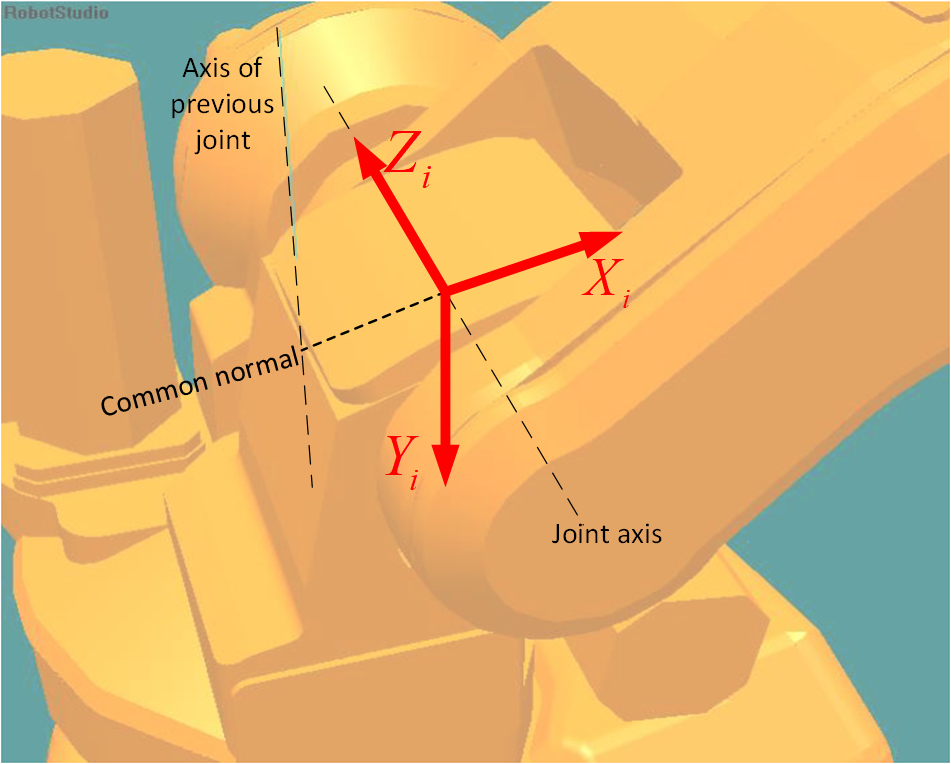
\includegraphics[
		width=1\linewidth,
		center,
		keepaspectratio,
		]{AssignationOfFrames/NonCoplanar}
		\caption{Example for non coplanar axes \cite{DenavitHartenbergKonventionen}}
		\label{fig:NonCoplanar}
%	\end{minipage}%
	\end{figure}
	\begin{figure}[H]
%	\begin{minipage}{.3\textwidth}
		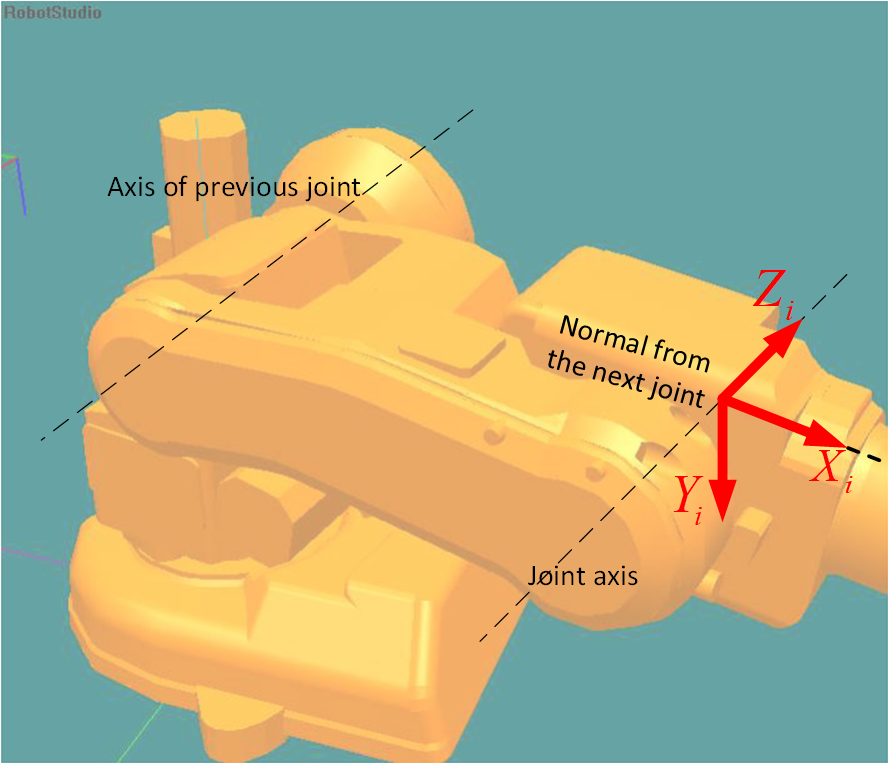
\includegraphics[
		width=1\linewidth,
		center,
		keepaspectratio,
		]{AssignationOfFrames/Parallel}
		\caption{Example for parallel axes \cite{DenavitHartenbergKonventionen}}
		\label{fig:Parallel}
%	\end{minipage}%
	\end{figure}
	\begin{figure}[H]
%	\begin{minipage}{.3\textwidth}
		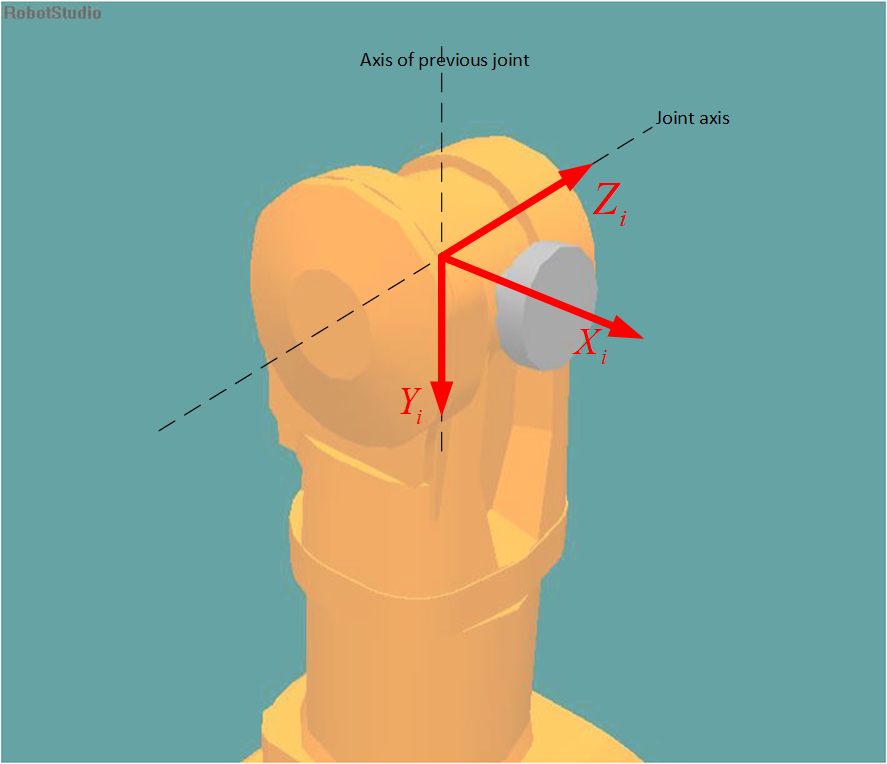
\includegraphics[
		width=1\linewidth,
		center,
		keepaspectratio,
		]{AssignationOfFrames/Intersecting}
		\caption{Example for intersecting axes \cite{DenavitHartenbergKonventionen}}
		\label{fig:Intersecting}
%	\end{minipage}%
	
\end{figure}